\begin{figure}[H]\centering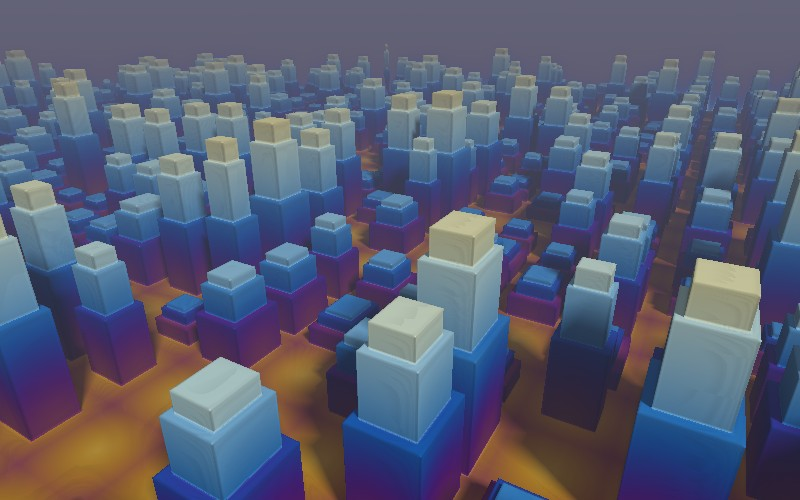
\includegraphics[width=0.88\textwidth]{img/skyline.jpg}
\caption{Skyline, default parameters (3 iterations).}\end{figure}
\paragraph{Parameters (app defaults).} Iterations 3 (range 1--5); step factor 0.8; bounding size 2; \emph{unbounded} (no bounding sphere assumed).

{\footnotesize\begin{tabular}{@{}llrr@{}}\toprule Parameter & Key & Default & Range\\\midrule
Block size & \texttt{cell} & 1 & 0.3\,\dots\,3\\
Height & \texttt{height} & 1.8 & 0.1\,\dots\,6\\
Height variety & \texttt{vary} & 0.75 & 0\,\dots\,1\\
Density & \texttt{density} & 0.8 & 0\,\dots\,1\\
Tower width & \texttt{width} & 0.32 & 0.15\,\dots\,0.42\\
Setback & \texttt{setback} & 0.25 & 0\,\dots\,0.8\\
Seed & \texttt{seed} & 7 & 0\,\dots\,100\\
\bottomrule\end{tabular}}
